\documentclass[]{article}

% Imports the catppuccin theme, using the mocha flavor,
% from the directory above. Actual implementation
% wouldn't need the import package unless the theme
% and the document are in different directories.
\usepackage{import}
\usepackage{xcolor}
% \usepackage{fancyhdr}
\usepackage{cancel}
\usepackage{mathtools}

% For permutations and combinations
\newcommand\Myperm[2][^n]{\prescript{#1\mkern-2.5mu}{}P_{#2}}
\newcommand\Mycomb[2]{\prescript{#1\mkern-0.5mu}{}C_{#2}}

% Colors
\definecolor{yorhabg}{HTML}{FFFFFF}
\definecolor{yorhafg}{HTML}{000000}
\definecolor{yorhagrid}{HTML}{B5AF9C}
\definecolor{mred}{HTML}{D67069}
\definecolor{mblue}{HTML}{6887A1}

\pagecolor{yorhabg}
\color{yorhafg}

\usepackage{preamble}

% Removes padding above title
\usepackage{titling}
\setlength{\droptitle}{-10em}

% Font package
\usepackage[T1]{fontenc}

\usepackage{fouriernc}

\usepackage{sectsty}
\usepackage{graphicx}
\usepackage{amsmath}
\usepackage{amsfonts}
\usepackage{amssymb}
\usepackage[skins, most]{tcolorbox}
\usepackage{enumitem}

\DeclareMathOperator{\sgn}{sgn}

\usepackage{tikz}
\usepackage{eso-pic}
\usetikzlibrary{calc,shadows.blur}
\usetikzlibrary{angles, quotes}
\usetikzlibrary{3d}

% Margins
\topmargin=0in
\evensidemargin=0in
\oddsidemargin=0in
\textwidth=6.5in
\textheight=9.0in
\headsep=0.25in

\AtBeginEnvironment{tcolorbox}{\small}

\newtcolorbox{imp}{enhanced,arc=0mm,colback=yorhabg,colframe=mred,leftrule=10mm,coltext=yorhafg,%
overlay={\node[anchor=west,outer sep=2pt] at (frame.west) {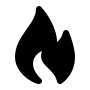
\includegraphics[width=6mm]{images/imageb.png}}; }}

\newtcolorbox{shortcut}{enhanced,arc=0mm,colback=yorhabg,colframe=mred,leftrule=10mm,coltext=yorhafg, coltitle=yorhabg, title=\texttt{Shortcut.}, 
overlay={\node[anchor=west,outer sep=2pt] at (frame.west) {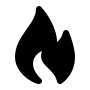
\includegraphics[width=6mm]{images/imageb.png}}; }}

\newtcolorbox{question}[1]{
    enhanced, 
    colback=yorhabg,
    colframe=mblue,
    coltext=yorhafg,
    coltitle=yorhabg,
    attach boxed title to top left={yshift*=-\tcboxedtitleheight}, 
    title=\texttt{#1},
    boxed title size=title,
    boxed title style={%
        rounded corners=northeast, 
        rounded corners=northwest, 
        colback=tcbcolframe, 
        boxrule=0pt,
    },
    underlay boxed title={%
        \path[fill=tcbcolframe] (title.south west)--(title.south east) 
            to[out=0, in=180] ([xshift=5mm]title.east)--
            (title.center-|frame.east)
            [rounded corners=5pt] |- 
            (frame.north) -| cycle; 
    },
}
% \pagestyle{fancy}
% \fancyhf{}  % Clear all default header/footer
% \fancyhead[L]{\small Satyajit Datta \\ 1012033336}  % Top-left, small font
\newcommand\bb[1]{\textcolor{yorhafg}{\textbf{#1}}}

\title{\textbf{CSCA67 - Exercises \#4}}
\author{Satyajit Datta \\ 1012033336}
\date{\today}

\begin{document}

\maketitle

For each of the following arguments, prove if they are valid or not.


\begin{question}{1.1}
Every insect has six legs. Charlotte has six legs. Therefore, Charlotte is an insect.

Let $I(x)$ be "$x$ is an insect". $L(x)$ be "$x$ has six legs. Universe of discourse is live beings.
\end{question}

The argument given is:
\begin{align*}
    & \forall x(I(x) \rightarrow L(x)) & (1)\\
    & L(Charlotte) & (2)\\
    & \overline{I(Charlotte)} & \text{(Conclusion)}
\end{align*}


\begin{question}{1.2}
Every insect has six legs. At least one insect flies. Therefore, at least one six-legged being flies.

Let $I(x)$ be "$x$ is an insect". $L(x)$ be "$x$ has six legs", $F(x)$ be "$x$ flies." Universe of discourse is live beings.
\end{question}
The argument given is: 
\begin{align*} 
    & \forall x(I(x) \rightarrow L(x)) & (1)\\ 
    & \exists x, (I(x) \land F(x)) & (2)\\ 
    & \overline{\exists x, (L(x) \land F(x))} & \text{(Conclusion)} 
\end{align*} 
\medbreak

\underline{\textbf{Proof.}}

\begin{flalign*}
  &\text{Take an element }c\text{ such that: }I(c)\land F(c) && (3)\ \text{(EI)}\\
  &\quad I(c) && (4)\ \text{(3, simp.)}\\
  &\quad F(c) && (5)\ \text{(3, simp.)}\\
  &\quad L(c) && (6)\ \text{(1, 4, Universal Modus Ponens)}\\
  &\quad L(c)\land F(c) && (7)\ \text{(5, 6, conj.)}\\
  &\exists x\,(L(x)\land F(x)) && (8)\ \text{(7, EG)}
\end{flalign*}
\hrule
\vspace{0.1in}
$\therefore$ The argument is valid. $\blacksquare$


\begin{question}{1.3}
Every insect has six legs. Only insects fly. Therefore, every flying being has six legs.

Let $I(x)$ be "$x$ is an insect". $L(x)$ be "$x$ has six legs, $F(x)$ be "$x$ flies." Universe of discourse is live beings.
\end{question}

The argument given is:
\begin{align*}
    & \forall x(I(x) \rightarrow L(x)) & (1)\\
    & \forall x, (F(x) \rightarrow I(x)) & (2)\\
    & \overline{\forall x, (F(x) \rightarrow L(x))} & \text{(Conclusion)}
\end{align*}

\begin{align*}
    &\text{Take an arbitrary}\; c &  \hfill & (3) \\
    &\quad 
\end{align*} 

\begin{question}{1.4}
All birds eat at least one species of insect. At least one species of insect can fly. Therefore, all birds
eat some flying being.

Let $I(x)$ be "$x$ is a species of insect.", $B(x)$ be "$x$ is a bird, $F(x)$ be "$x$ flies.", and $E(x,y)$ be "$x$ eats $y$". Universe of discourse is live beings.
\end{question}

The argument given is:
\begin{align*}
    & \forall x\;(B(x) \rightarrow \exists y(I(y) \land E(x, y))) & (1)\\
    & \exists x, (I(x) \land F(x)) & (2)\\
    & \overline{\forall x, (B(x) \rightarrow \exists y(F(y) \land E(x, y)))} & \text{(Conclusion)}
\end{align*}

\end{document}
